
\subsubsection{Applied Algorithms}\label{ict:robotics:carpin}
\index{Carpin, Stefano}
\paragraph{Research Team}
Stefano Carpin (Professor), Hamed Bastani (PhD Student), Gorkem Erinc (MSc Student), Andreas Kolling (MSc Student)\\

The main research focus is on the computational aspects of
robotics, with a special emphasis on motion planning and
cooperative tasks. By their very own nature, robots are machines
that execute their tasks in the physical world. Their control
algorithms have then to consider physical laws and constraints,
and process noisy information acquired during their execution.
This unique combination of challenges calls for the design of
algorithmic techniques that bring together computer science,
control theory, probability and computational geometry. Another area of active
research is on the development of tools for the realistic
simulation of robot systems, with special attention to multi-robot
systems. The goal in this case is to produce the tools for a fast
development of robot algorithms.


\paragraph{Highlights}

During the year 2006 a major effort has been spent to perfect
and promote the USARSim simulator. This project, jointly
developed with the National  Institute of Standards and Technology (USA)
and the University of Pittsburgh is experiencing significant
popularity and is rapidly becoming one of the most widely
used robot simulators (packages composing the software have
been downloaded more than 6000 times). The software
provides an ideal experimental environment to perform early
validation of robot algorithms for tasks like planning, navigation,
exploration, mapping and the alike. The simulator has been adopted
as software infrastructure for a new Robocup competition held
for the first time during the 2006 event held in Bremen. During the
competition, the IUB team led by Prof. Carpin won the second place.

Continuing a well established vein of research in cooperative
multi-robot systems, a new solution for the Cooperative Multi-robot
Observation of Multiple Moving Targets (CMOMMT) has been proposed.
The designed algorithm overcomes some of the deficiencies found in
formerly suggested approaches by introducing explicit communication
between the pursuer robots, as well as motion prediction mechanisms
that are not programmed a priori, but rather learned by the system.
This investigation led to the discovery of more additional fundamental
research topics that are currently being pursued. Applications
in the long term can be envisioned in the field of assisted surveillance.

Finally, a novel algorithm for determining the translation collision
distance between convex polyhedra has been developed. The problem of
distance computation is fundamental in tasks like motion planning,
virtual prototyping and computer aided design. The proposed
algorithm exhibit interesting properties. It performs well both on
computations where no prior information is available, but it can
also favorably exploit prior knowledge obtained from formerly
resolved problem instances (so called {\em incremental computation}.
Comparisons with state of the art alternatives outline better
asymptotic trends (Figure~\ref{fig:Carpin_pic1} shows and example of
comparative results with other algorithms).



\begin{figure}[ht]
\begin{center}
     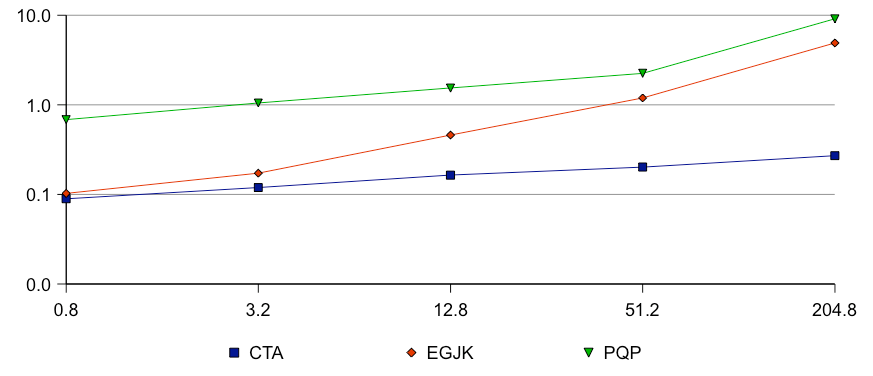
\includegraphics[width=\hsize]{Carpin_Figure_CTA.pdf}
    \mycaption{Time spend to solve a collision query as a function of
    the complexity of the involved polyhedra. The blue line outlines
    the performance of the proposed algorithm.}
    \label{fig:Carpin_pic1}
\end{center}
\end{figure}





\paragraph{Organization}

\begin{enumerate}
    \item 6th IEEE International Workshop on Robot Motion and  Control: program committee
          member
   \item IEEE 2006 International Conference  on Information Reuse  and
Integration: program committee member
\item PerMIS 2006: program committee member
   \item 6th international joint conference on autonomous agents and multiagent
          systems: program committee member
\item Robocup Federation: elected Executive Member for the 2007-2009 term
\item Organizer of  a tutorial on "USARSim/MOAST: Highly Realistic Simulation and Control for Multi Robot" held at the IEEE International
Conference on Robotics and Automation (Orlando-FL, May 2006)
\item Organizer of a tutorial on "USARSim and MOAST: Advanced Tools for High-Fidelity Simulation of Distributed Robot Systems "   held at the annual conference
of the American Association for Artificial Intelligence  (Boston-MA, July 2006)
\end{enumerate}

\paragraph{Collaborations}
\begin{enumerate}
    \item {\sl National Institute of Standards and Technology, USA}\\
          Dr. Steve Balakirski\\
          Organization of the Virtual League Competion and development of USARSim
    \item {\sl University of Pittsburgh, USA}\\
          Prof. Mike Lewis\\
          Organization of the Virtual League Competion
    \item {\sl University of Udine, Italy}\\
          Prof. Claudio Mirolo\\
          Development of Algorithms for Collision Detection
    \item {\sl University  of Padova, Italy}\\
          Prof. Enrico Pagello\\
          Development of Algorithms for Multi-Robot Motion Planning
\end{enumerate}



%\paragraph{Publications}

%\begin{description}
 % \item[Journals]
 \nocite{Carpin:IEEEPRO2006}\nocite{Carpin:ACTA2006}\nocite{Carpin:AR2006}

 % \item[Conference Proceedings]
  \nocite{Carpin:IAS2006}\nocite{Carpin:RS1}\nocite{Carpin:RS3}
  \nocite{Carpin:PerMIS2006b}\nocite{Carpin:PerMIS2006a}\nocite{Carpin:ICRA2006GM}
  \nocite{Carpin:ICRA2006BCMOMMT}
 % \item[Books/Collections]
   \nocite{Carpin:LNCS4123}
%\end{description}
%\end{document}
%%% Local Variables:
%%% mode: latex
%%% TeX-master: "report"
%%% End:
